\documentclass[12pt]{article}
\usepackage{amssymb, amsmath}
\usepackage{bm}
\usepackage{dsfont}
\usepackage{empheq}
\usepackage{graphicx}
\usepackage{float}

% Set up the margins.
\usepackage[top=1in, bottom=1in, left=1in, right=1in]{geometry}


\begin{document}


\section{Probabilistic Graphical Models 1: Representation}

\subsection{Week 1. Introduction and Overview}

Please see the student example in Fig.~\ref{fig:student_example}.

\begin{figure}[H]
\centering
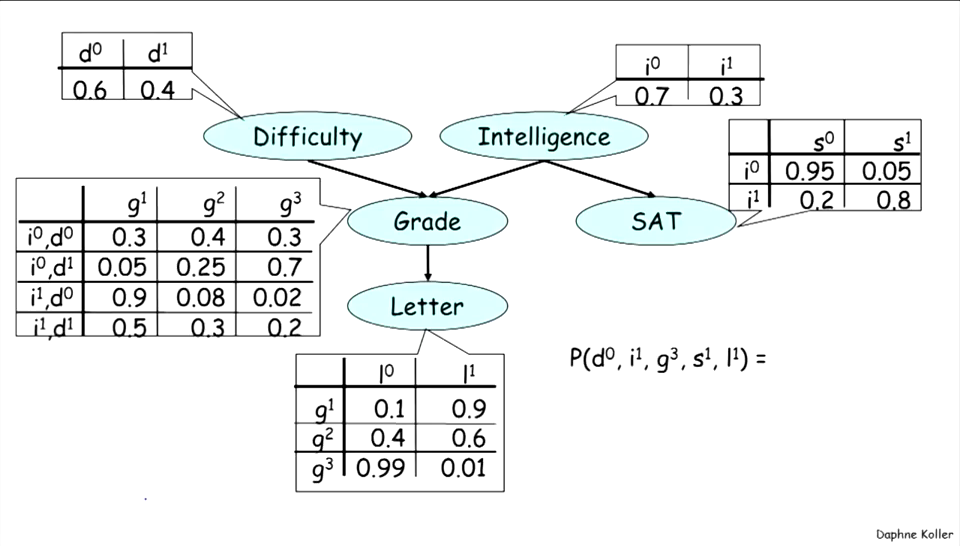
\includegraphics[width=6in]{graphics/student_example.png}
\caption{Student Example.}
\label{fig:student_example}
\end{figure}


\begin{itemize}
    \item Grade ($G$) --- $g^1(A)$, $g^2(B)$, and $g^3(C)$.
    \item Course Difficulty ($D$) --- $d^0(\text{easy})$, $d^1(\text{hard})$.
    \item Student Intelligence ($I$) --- $i^0(\text{low})$ and $i^1(\text{high})$.
    \item SAT score ($S$).
    \item Reference Letter ($L$).
\end{itemize}
 

% D, I --> G --> L
% I --> S


\subsubsection{Joint Distribution}
Consider $\Pr(I, D, G)$.

\subsubsection{Conditioning}
For example, we can condition on $G=g^1$.  We look at $\Pr(I, D, g^1)$.
We need to renormalize. That is
\begin{equation*}
  \Pr(I, D | g^1) = \frac{\Pr(I, D, g^1)}
                         {\sum_{I=i^j} \sum_{D=d^k} \Pr(I, D, g^1)}  \, .
\end{equation*}
The above equation comes from the definition of conditional probability $\Pr(A | B) = \Pr(A, B) / \Pr(B)$.

\subsubsection{Marginalization}
For example, we marginalize $I$.

\begin{equation*}
  \Pr(D) = \sum_{I=i^j} \Pr(I, D)
\end{equation*}

\subsection{Week 1. Bayesian Network (Directed Models)}


Chain rule:
\begin{equation}
  \Pr(D, I, G, S, L) = \Pr(D) \Pr(I) \Pr(G|I, D) \Pr(S|I) \Pr(L|G)
\end{equation}

\begin{equation}
  \Pr(X_1, ..., X_n) = \prod_i \Pr(X_i | \text{Par}_\mathbb{G}( X_i ) ) \, ,
\end{equation}
where $\text{Par}_\mathbb{G}( X_i )$ are the parents of $X_i$ over the graph $\mathbb{G}$.

% ---

% Causal reasoning
% e.g., Pr(L = 1 | I = 0) = 0.39

% Evidential reasoning (from the bottom up)
% e.g., Pr(D = 1 | G = 3) = 0.63

% Intercausal reasoning
% e.g., Pr(I = 1 | G = 2, D = 1) = 0.34

% e.g., Let Y = (X_1 or X_2)
% Pr(X_2 = 1 | Y = 1) = 2/3, but
% Pr(X_2 = 1 | Y = 1, X_1 = 1) = 1/2

% ---

% Conditional independence

% Example.  Tossing a coin twice, which might be fair or not.

% C --> X_1, X_2.

% Pr(X_2 = H | X_1 = H) > 0.5 because the coin might not be fair.

% However, Pr(X_2 = H| C = coin) is indep of X_1!

% In her notation,
%   P does NOT satisfy X_1 perpendicular X_2
%   P satisfies (X_1 perpendicular X_2 | C)

% Conditioning can remove independence.

% However, conditioning can also introduce independence.
% I, D --> G

% Look at Pr(I, D| G = 1).  It couples I and D.

% ---

% Pr(X, Y) = Pr(X) Pr(Y) if X, Y are indep.

% Pr(X, Y, Z) ~ phi_1(X, Z) phi_2(Y, Z) if (X perpendicular Y | Z)

% ---

% Any node is d-separated from its non-descendants given its parents.

% In other words, if P factorizes over G, in P, any variable is independent of its non-descendants _given_ its parents.

% ---

% I-map (independency map)

% I(G) = { (X perpen Y | Z) : d-sep_G(X, Y | Z) }



\end{document}
